% Created 2020-05-19 Tue 10:26
% Intended LaTeX compiler: pdflatex
\documentclass[11pt]{article}
\usepackage[utf8]{inputenc}
\usepackage[T1]{fontenc}
\usepackage{graphicx}
\usepackage{grffile}
\usepackage{longtable}
\usepackage{wrapfig}
\usepackage{rotating}
\usepackage[normalem]{ulem}
\usepackage{amsmath}
\usepackage{textcomp}
\usepackage{amssymb}
\usepackage{capt-of}
\usepackage{hyperref}
\usepackage{listings}
\date{\today}
\title{Return Oriented Program Evolution with ROPER}
\hypersetup{
 pdfauthor={},
 pdftitle={Return Oriented Program Evolution with ROPER},
 pdfkeywords={},
 pdfsubject={},
 pdfcreator={Emacs 26.3 (Org mode 9.3.6)}, 
 pdflang={English}}
\begin{document}

\maketitle
\setcounter{tocdepth}{1}
\tableofcontents


\section*{}
\label{sec:orge4c8563}

\section*{Introductory Remarks}
\label{sec:orgb3a58ba}
\section*{The Concept of Return-Oriented Programming}
\label{sec:orgdb9113f}
\subsection*{The Fundamental Problem of Cybersecurity}
\label{sec:orgab4ab0a}
At bottom, there is no essential distinction between data and code.

"Data" is just information your system trusts. 
\subsection*{The Stack}
\label{sec:org81a5540}
\begin{center}
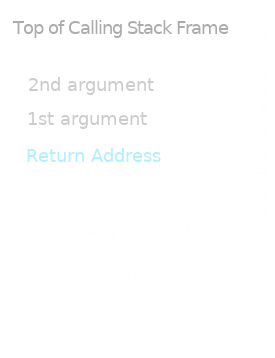
\includegraphics[width=.9\linewidth]{./img/stack_frame.png}
\end{center}
\begin{itemize}
\item the hacker feeds some input data to the process
\item which is written to a buffer in stack memory
\item but which overruns the buffer
\item corrupting the frame's return address
\end{itemize}

\subsection*{The Stack, Smashed}
\label{sec:orgab47018}

\begin{center}
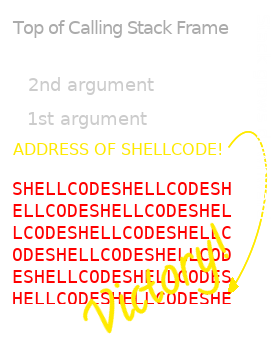
\includegraphics[width=.9\linewidth]{./img/stack_frame_attack.png}
\end{center}
\begin{itemize}
\item so that it points into the buffer
\item a buffer that turns out to contain machine code
\item to which the program counter "returns"
\item executing it just as it would its own instructions!
\end{itemize}

\subsection*{\(\textit{DEP}~~/~~W \oplus X\)}
\label{sec:org3d69e93}
\begin{center}
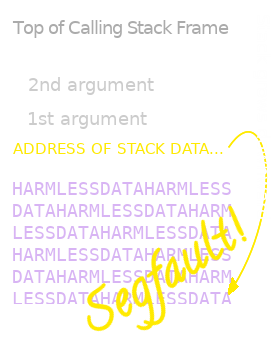
\includegraphics[width=.9\linewidth]{./img/stack_frame_attack_w^x.png}
\end{center}
\begin{itemize}
\item One way of mitigating this is to try to ensure that no page of memory is both writeable \textbf{and} executable.
\item The idea being that \emph{data} should be writeable, but never executable, while \emph{code} should be executed, but not written at runtime.
\end{itemize}


\subsection*{Subverting \(~~W\oplus X\)}
\label{sec:org7af5343}
\begin{itemize}
\item \(W\oplus X\) may prevent the \emph{execution} of input data, but it doesn't prevent attempts to \emph{return} to that data.
\item Why should the hacker need to supply their own machine code?
\item There's quite a bit just laying around, in executable memory.
\item Why not just build a payload with whatever's handy?
\end{itemize}
\subsection*{\(W\oplus X~~\) is a Leaky Abstraction}
\label{sec:orgc6d633d}
\begin{itemize}
\item It rests on all-too-narrow concepts of "instruction" and "execution".
\item The payload's \emph{instructions} don't need to be bytes of machine code.
\item They just need to influence control flow, in a controllable way.
\end{itemize}
\subsection*{So is the \emph{Structured Programming Machine Model}}
\label{sec:orgc3052a8}
\begin{itemize}
\item The machine model on which structured programming is based already carves up an executable into chunks that \textbf{return} control after being dispatched.
\item To the programmer, these are "functions", but this is too granular a viewpoint.
\item \emph{Any} chunk of code ending with a \textbf{return} returns control to whomever controls the stack.
\item And our data controls the stack!
\end{itemize}

\subsection*{The ROVM supervenes on the SPMM}
\label{sec:org2c68d29}
\begin{center}
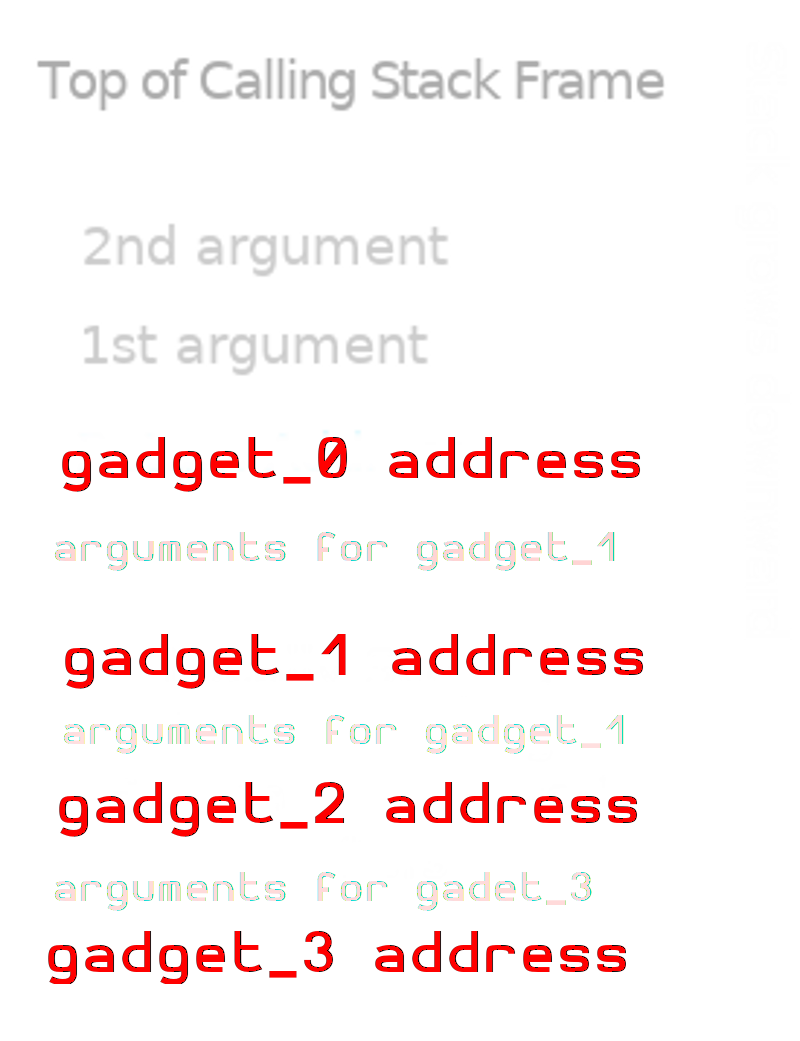
\includegraphics[width=.9\linewidth]{./img/stack_frame_rop.png}
\end{center}
\begin{itemize}
\item Chunks of code that return control are called "gadgets".
\item They form a spontaneous ISA, whose \textbf{program counter} is the \textbf{stack pointer} of the underlying architecture.
\item Let's call this ISA a "Return-Oriented Virtual Machine".
\end{itemize}

\subsection*{We can program this machine with input data}
\label{sec:orgfdea52d}
\begin{itemize}
\item All we need to do is to discover and supply a buffer of instructions.
\item These are not instructions for the underlying architecture, but for the ROVM.
\item \(W\oplus X\) is blissfully unaware of the ROVM, and powerless to prevent us from executing data as \emph{ROVM} code.
\end{itemize}

\section*{Genetic Programming}
\label{sec:org6618c18}
\subsection*{{\bfseries\sffamily TODO} Genetic Algorithms}
\label{sec:orgde0c582}
\begin{itemize}
\item Variation (mutation and crossover)
\item Selection (fitness function)
\item Reproduction (iteration)
\end{itemize}

\subsection*{Genotype \(\rightarrow\) Phenotype}
\label{sec:org9a2ab4d}

\begin{itemize}
\item Genetic programming turns on an analogy between genotype \(\rightarrow\) phenotype maps on the one hand, and, on the other, the relation between a program's syntax and its operational semantics.
\item The syntactical representation of a program is its genotype, and its semantic behaviour is its phenotype.
\end{itemize}

\subsection*{Exploring Weird Machines through Genetic Programming}
\label{sec:orgfc588dd}

\begin{itemize}
\item We are often going, blind, into terra incognita.
\item Evolutionary computation has shown surprising creativity
in discovering and exploiting computational environments.
(See \href{https://arxiv.org/abs/1803.03453}{The Surprising Creativity of Digital Evolution} for examples.)
\item The irregular, side-effect-rich character of the computational primitives
exposed by many WMs, ROP included, make them difficult for humans to reason about.
\end{itemize}

\subsection*{Challenges that ROP exploration poses for GP}
\label{sec:orgce7f464}

\begin{itemize}
\item GP typically employs highly specialized and parsimonious virtual machines,
tailored to the problem set in question.
\item Our "instruction set" is the set of "gadgets" we happen to discover in a binary.
\item This set is not small (often numbering in the hundreds, or more).
\item Nor "tailor made".
\item Nor is it evenly distributed over the semantic space it represents.
\end{itemize}


\section*{Design and Implementation of ROPER}
\label{sec:orgfa9285c}

\subsection*{Bird's eye view}
\label{sec:orgf630d43}
\begin{center}
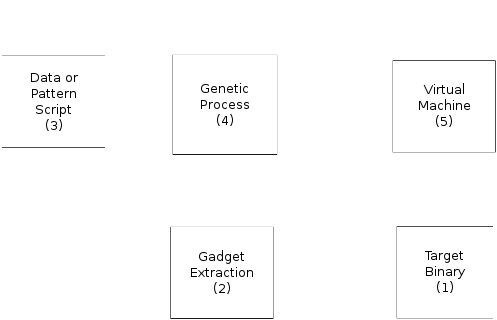
\includegraphics[width=.9\linewidth]{./img/birdseye_white.png}
\end{center}

\subsection*{Tournament Selection}
\label{sec:org4bc110a}
\begin{center}
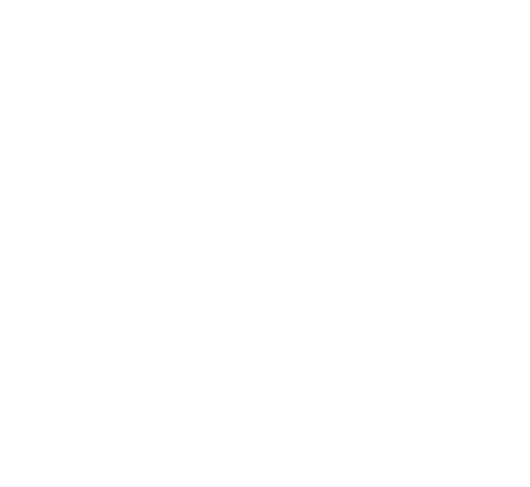
\includegraphics[width=.9\linewidth]{./img/tournament.png}
\end{center}

\subsection*{Genomic Structure}
\label{sec:org74c4c38}
\begin{itemize}
\item Each genome is a one-dimensional \emph{chain} composed of \emph{clumps}.
\item A \emph{clump} is a gadget address \(a\), followed by \(\texttt{SP}_\Delta(a)-1\) machine words
\item where \(\texttt{SP}_\Delta(a)\) is the (estimated) number of words that \(*a\) will pop from the stack, when run.
\item Several "epigenetic" fields of metadata are also associated with both the \emph{chain} and \emph{clump} structures.
\end{itemize}

\subsection*{Genetic Operators: Clumpwise Mutation}
\label{sec:org061d8fc}
\begin{itemize}
\item address substitution
\item arithmetical \& logical manipulation of dwords
\item indirection/dereference of dwords
\item permutation of pairs of dwords
\end{itemize}

\subsection*{Genetic Operators: Chainwise Crossover}
\label{sec:org3e94750}
\begin{itemize}
\item restricted to single-point crossover
\item splice point selected by weighted random choice, using the average of each link's previous hosts' fitness scores, to favour adaptive gene linkage
\item recently, a mechanism to promote homologous crossover in fitter specimens has been introduced
\end{itemize}


\section*{Experimental Studies}
\label{sec:org477ad50}

\subsection*{Tasks and Fitness Functions}
\label{sec:org57b2696}
\begin{itemize}
\item An arbitrary and inscrutable fitness function
\item System call preparation
\item Classification tasks:
\begin{itemize}
\item An artificial, linearly-separable dataset
\item The Iris dataset
\end{itemize}
\item A Snake game
\end{itemize}

\subsubsection*{System Call Preparation}
\label{sec:orgc87d45e}

\begin{itemize}
\item The goal here is to prepare the CPU for a system call, with the registers containing and pointing to the necessary arguments.
\item The fitness function uses a combination of numerical distance and bitwise hamming distance, for immediate values, and memory proximity for indirect values.
\item A successful evolutionary run delivers a payload that can be used for practical purposes.
\end{itemize}


\subsubsection*{System Call Preparation}
\label{sec:org4bf21c1}

Champion of the \emph{Wiwzuh} population:
\lstset{language=asm,label= ,caption= ,captionpos=b,numbers=none}
\begin{lstlisting}
  0000b4ac        pop {r4, r5, r6, r7, r8, pc}

  0000d1a0        cmp r0, #0
  0000d1a4        popeq {r3, r4, r5, pc}

  00016654        cmp r0, #0
  00016658        ldr r3, [pc, #4]
  0001665c        moveq r0, r3
  00016660        pop {r3, pc}

  0001706c        ldm sp, {r0, r1}
  00017070        add sp, sp, #0x10
  00017074        pop {r4, r5, r6, pc}

;; R0:  0001f62f   R2:  00000000
;; R1: &0001f62f   R7:  0000000b

;; to call execv("/tmp/flashXXXXXX", ["/tmp/flashXXXXXX"], NULL) 
  00018fc4        svcvc #0xffffff
\end{lstlisting}

\subsubsection*{Historical Profile of the \emph{Wiwzuh} population}
\label{sec:orgd0271fc}
\begin{center}
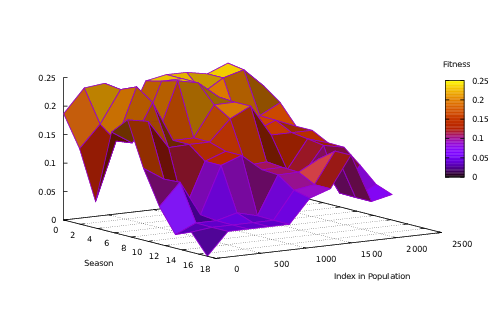
\includegraphics[width=.9\linewidth]{./img/wiwzuh_syscall_gaussian_3.png}
\end{center}

\subsection*{The Enigma of Stray Gadgets}
\label{sec:org870b934}
\begin{itemize}
\item This task also produced a number of specimens whose traces are too long and complex to display in detail here, but which were especially interesting for their labyrinthine nature, and the degree to which their execution traces strayed from the harvested gadget set.
\item I will nevertheless \textbf{try} to display one here.
\end{itemize}

\subsubsection*{The Enigma of Stray Gadgets}
\label{sec:orga65dca2}

\subsubsection*{The Enigma of Stray Gadgets}
\label{sec:org4b3f558}
These were of interest in two respects:

\begin{itemize}
\item they contained complex \emph{heuristic breakers} making them likely to bypass various IDS systems in the literature, as a sheer evolutionary \emph{spandrel}
\item theoretically, their behaviour was enigmatic. Straying is dangerous for chains, and comes with great risk of crashing, yet it appeared with \emph{prima facie} improbable frequency in our populations.
\end{itemize}

\subsection*{The Environment}
\label{sec:org1f8fa4b}
\begin{center}
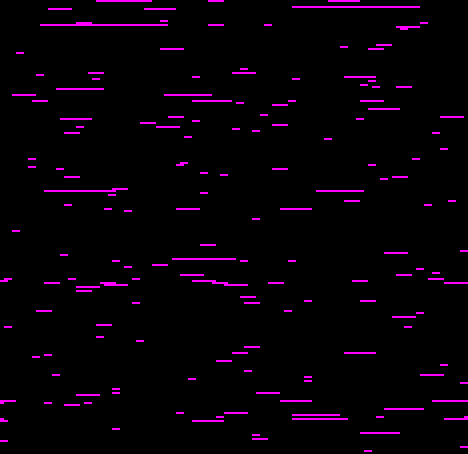
\includegraphics[width=.9\linewidth]{./img/tomato-RT-N18U-httpd_heatmap.png}
\end{center}

Distribution of gadgets in \texttt{tomato-RT-N18U-httpd}.

\subsection*{The Use of the Environment}
\label{sec:orgb5bfec0}
\begin{center}
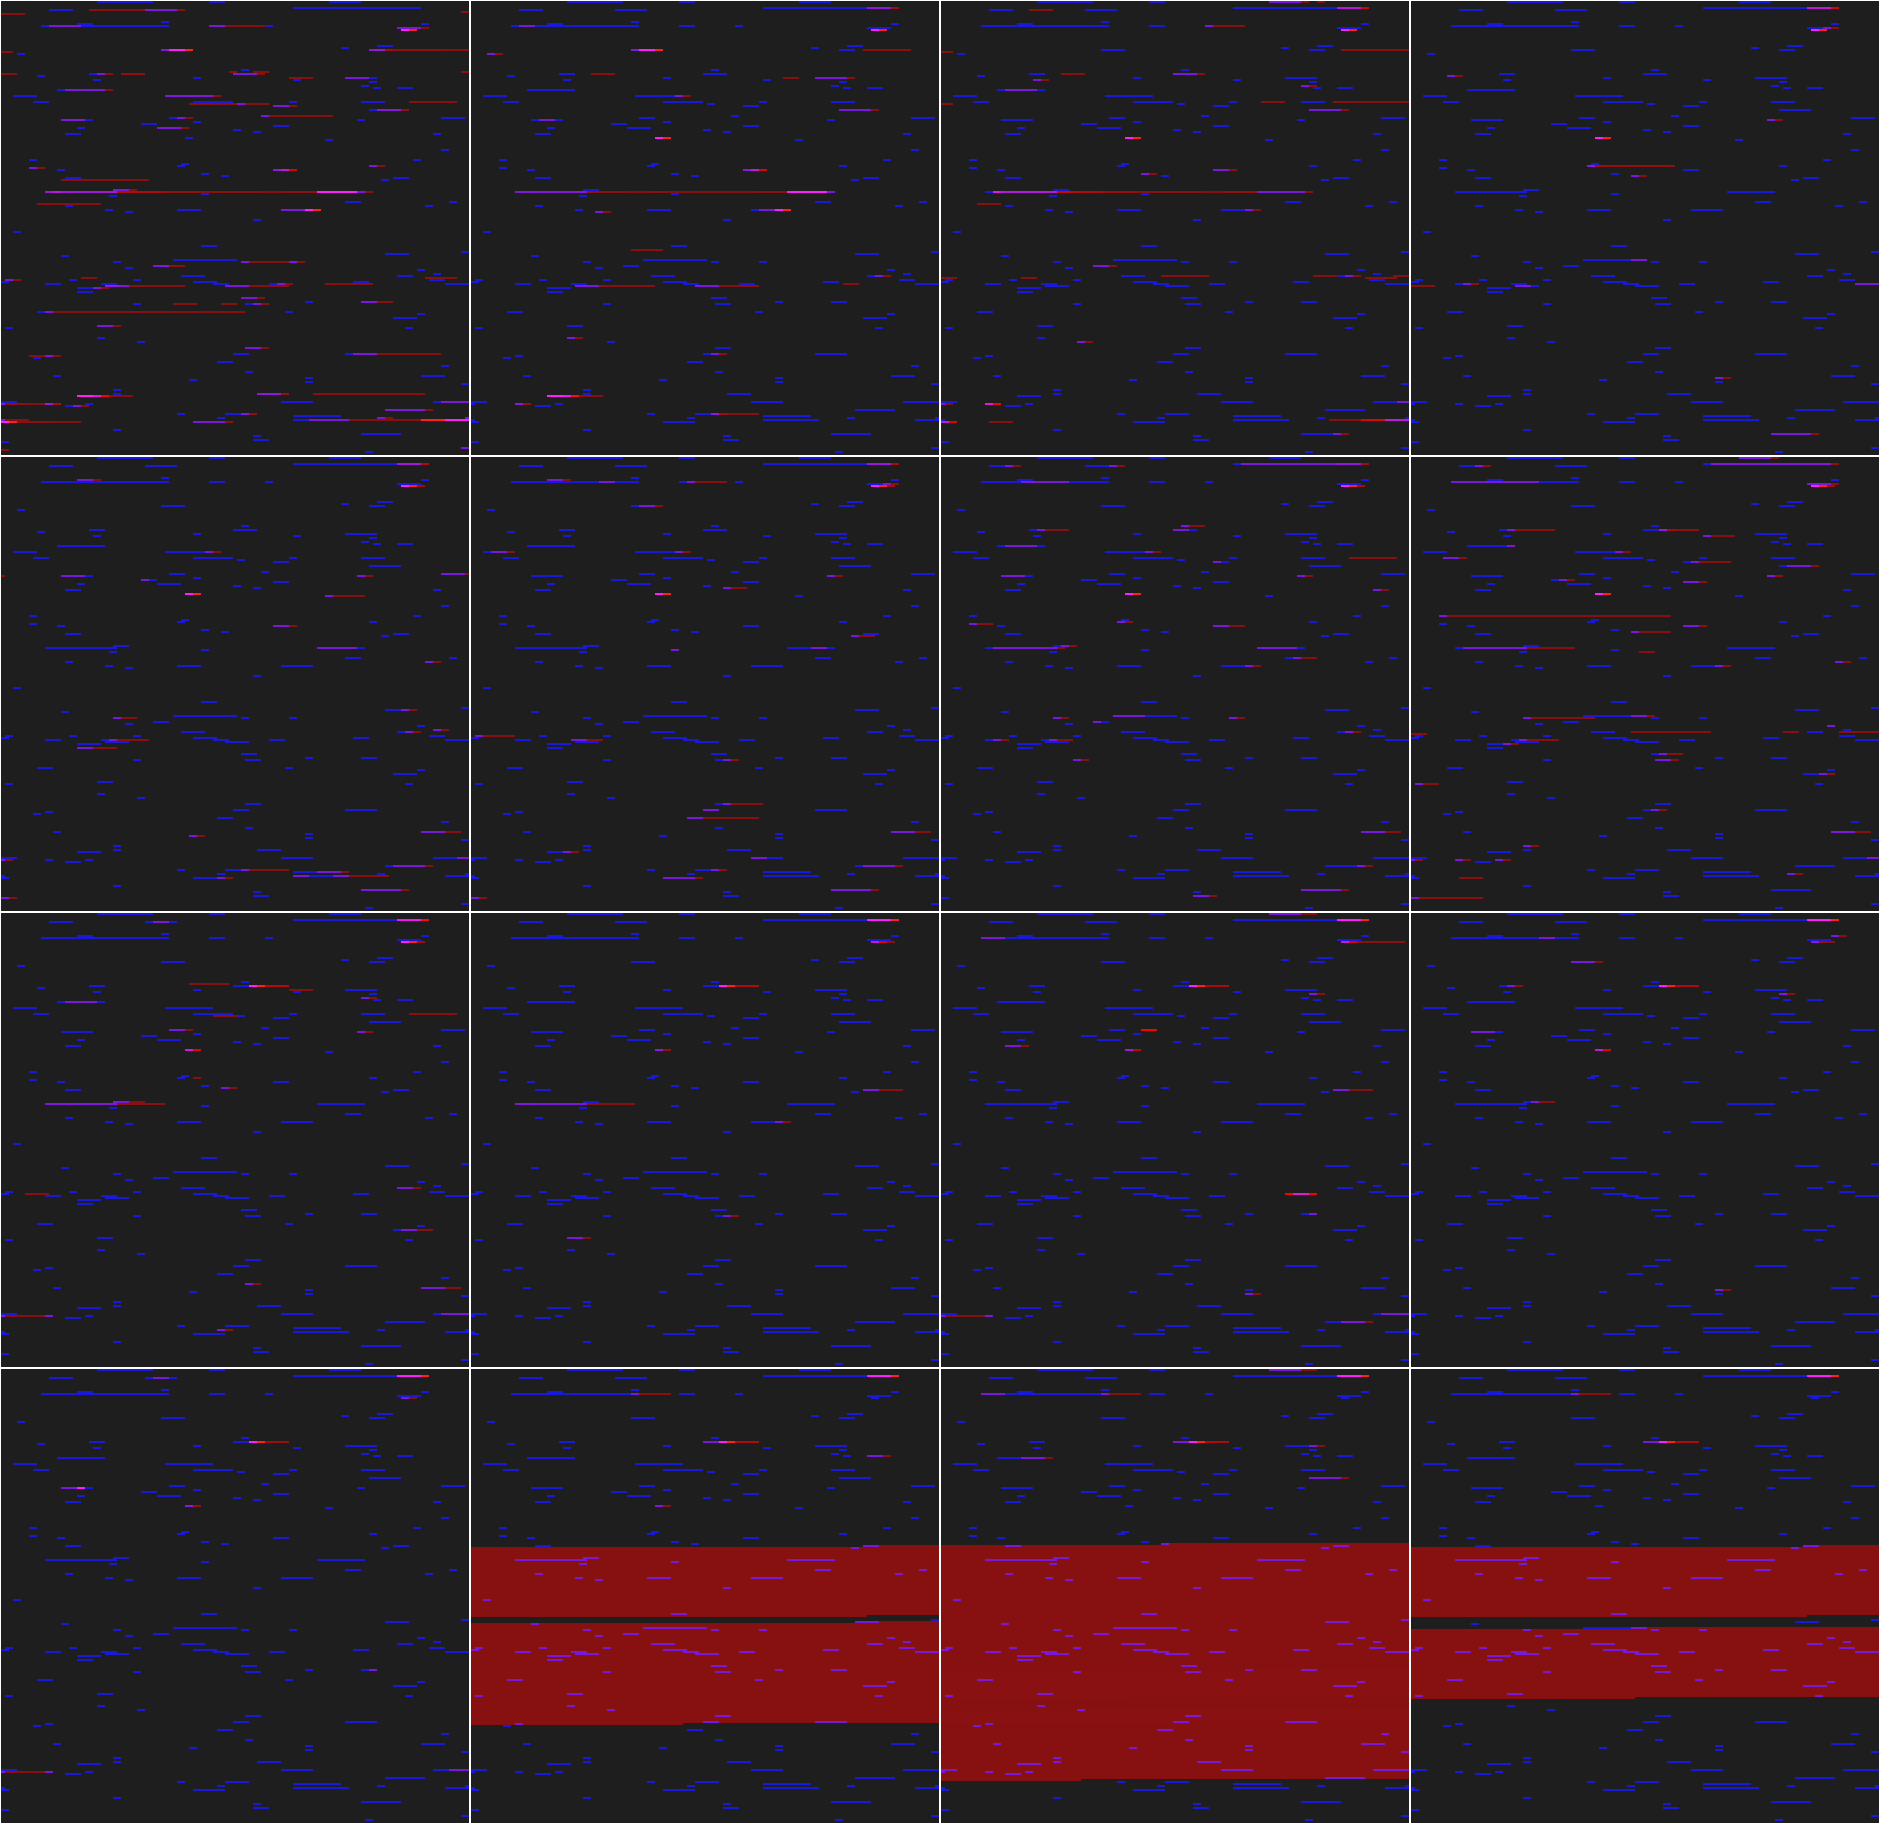
\includegraphics[width=.9\linewidth]{./img/fimjek_heatmap_montage.png}
\end{center}


\subsection*{A simple classification task}
\label{sec:org18386ec}
\begin{itemize}
\item For the classification tasks, I initially used a common, bid-based algorithm to map behaviour to classification decisions on data samples.
\item A set of output registers was mapped to the class list, and data was classified according to the register containing the greatest signed value.
\end{itemize}

\subsubsection*{Fair initial results}
\label{sec:orgb53082a}
\begin{center}
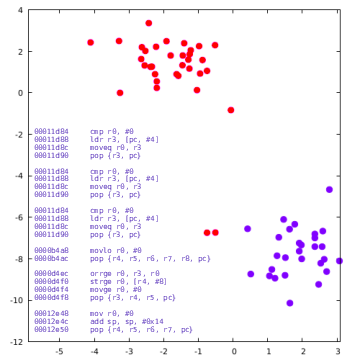
\includegraphics[width=.9\linewidth]{./img/kathot_champion.png}
\end{center}

\subsubsection*{An interesting case of malignancy}
\label{sec:org7bc3b44}

\begin{center}
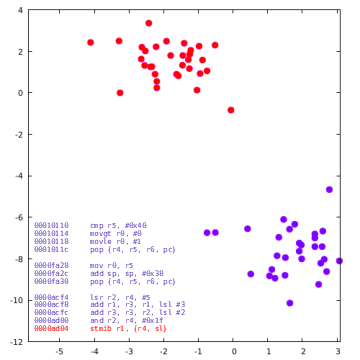
\includegraphics[width=.9\linewidth]{./img/fizwej_perfect_crash.png}
\end{center}

Here, the gene responsible for correct classification of the data was also responsible for crashing the execution. It rapidly took over the population.

\subsubsection*{An interesting case of malignancy}
\label{sec:orgf16cc07}
\begin{center}
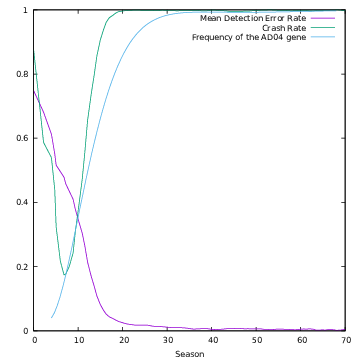
\includegraphics[width=.9\linewidth]{./img/fizwej-badgenes.png}
\end{center}

\subsubsection*{The Iris Dataset}
\label{sec:org85dea46}
\begin{center}
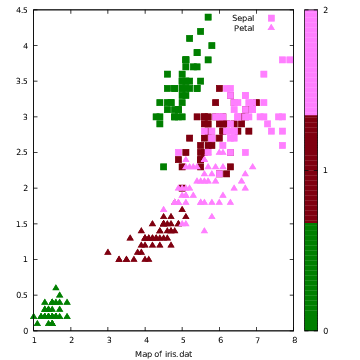
\includegraphics[width=.9\linewidth]{./img/iris_plot.png}
\end{center}

\subsubsection*{ROPER on the Iris Dataset}
\label{sec:org2b1fb00}
\begin{itemize}
\item This dataset proved a serious challenge for ROPER, which rarely achieved better than a 66\% detection rate (using the bid-bin method).
\item Success only came with the introduction of a fitness sharing mechanism.
\end{itemize}

\subsubsection*{Iris without Fitness Sharing}
\label{sec:orga49eb9b}
\begin{center}
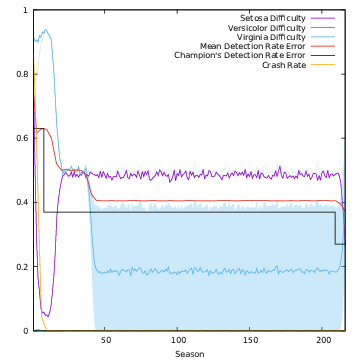
\includegraphics[width=.9\linewidth]{./img/nosharing.png}
\end{center}

\subsubsection*{Iris with Fitness Sharing}
\label{sec:org2160a44}
\begin{center}
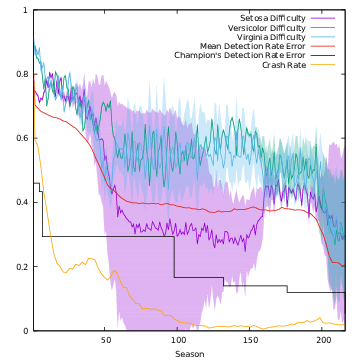
\includegraphics[width=.9\linewidth]{./img/sharing.png}
\end{center}

\subsubsection*{Iris as Classified by ROPER}
\label{sec:orgfb5fa40}
\begin{center}
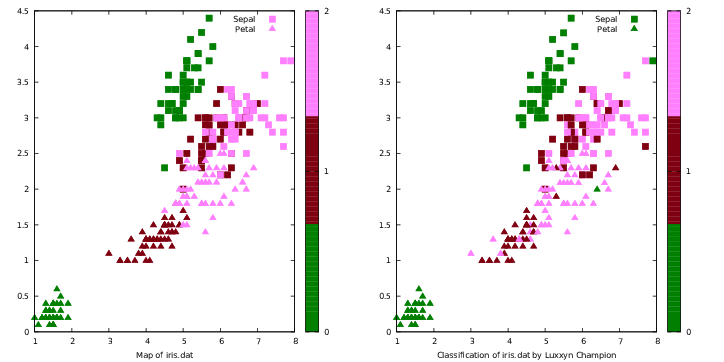
\includegraphics[width=.9\linewidth]{./img/iris_with_luxxyn.png}
\end{center}

\section*{Questions?}
\label{sec:orgbc98356}
\end{document}